\defChapterTarget{Graphical representations}
    Di seguito vengono riportate le cardinalità dei vari "Kind of Topic" e delle
    relazioni tra di loro:
    \begin{itemize}
        \item \textbf{Servizi}: In questa categoria ricadono le principali
        attività che vengono svolte dall'associazione durante gli orari di
        lavoro con frequenza giornaliera o settimanale. La cardinalità N dei
        servizi dovrebbe stare su un intorno del centinaio di elementi, prese in
        considerazione tutte le materie esistenti di cui fare ripetizioni e
        tutti i possibili orientamenti su tutti i diversi gradi di istruzione;
        \item \textbf{Persone}: Data la natura dell'associazione, si definisce
        volontario (e quindi elemento da inserire a sistema), una persona che ha
        la possibilità di partecipare attivamente ai servizi dell'associazione.
        Questa analisi comporta un'evidente necessità di vicinanza geografica,
        ergo la cardinalità N indicata in figura è direttamente proporzionale
        all'estensione territoriale. Per motivi ovvi, l'assunzione del sito
        Ripe4U è quella di una sola sede sul territorio milanese, ergo non si
        supereranno i 30 volontari;
        \item \textbf{Eventi}: Nella categoria "Eventi" ricadono tutte quelle
        attività proposte dall'associazione per i propri volontari, e non, che
        avvengono con frequenza mensile o semestrale. A fronte di queste
        considerazioni, la cardinalità di questo Kind of Topic difficilmente
        supererà le 30 unità;
        \item \textbf{Servizi -> Eventi}: La relazione esprime, dato un servizio
        X, tutti gli eventi durante il quale è possibile trovare quel dato
        servizio. Prenderemo, pertanto, il caso pessimo, ovvero quando un
        servizio è presente in tutti gli eventi che l'associazione propone. La
        cardinalità di N, visti i presupposti, è in questo caso pari alla
        cardinalità dell'insieme totale degli eventi proposti;
        \item \textbf{Eventi -> Servizi}: Si esprime con questa relazione tutti
        quanti i servizi presenti all'interno di un evento che, nel caso di una
        vacanza studio dovrebbe aggirarsi (per questioni logistiche e
        temporali), in un intorno di 10 servizi per evento.
    \end{itemize} 
    \section{C-IDM} 
    \begin{figure}[H]
        \centering
        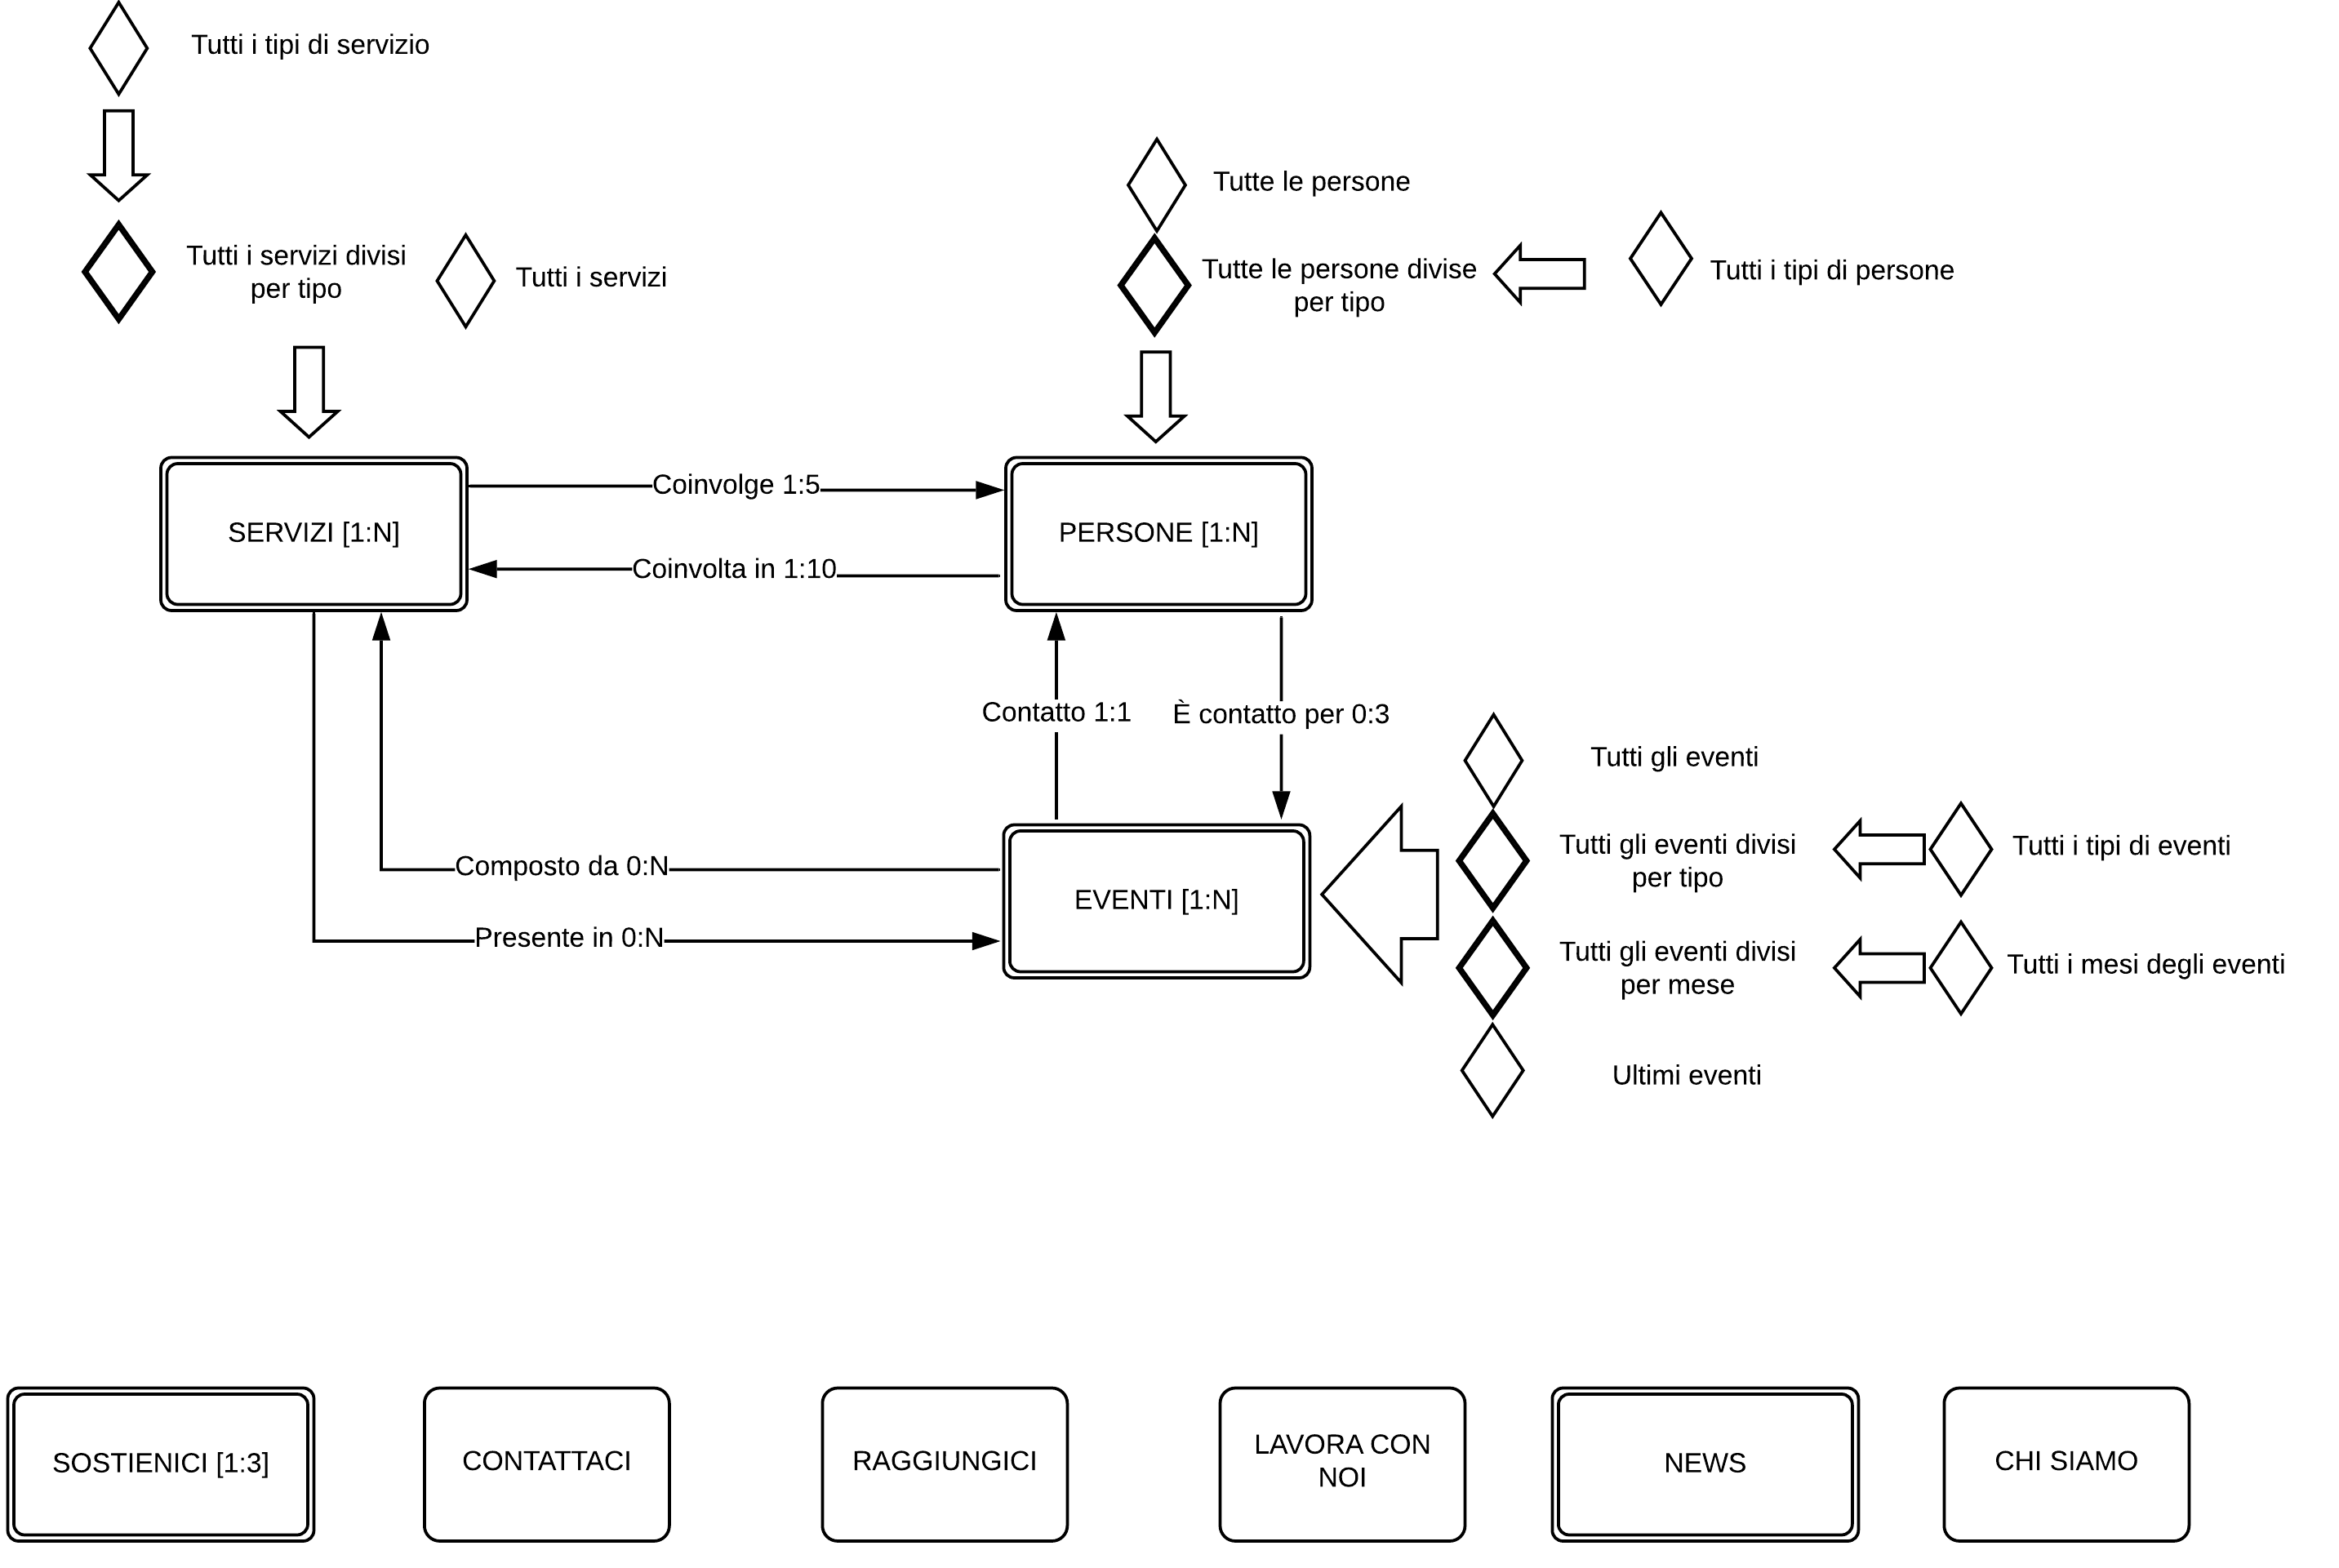
\includegraphics[scale=0.6]{resources/images/c-idm.png}
    \end{figure}
    \section{L-IDM}
    \begin{figure}[H]
        \centering
        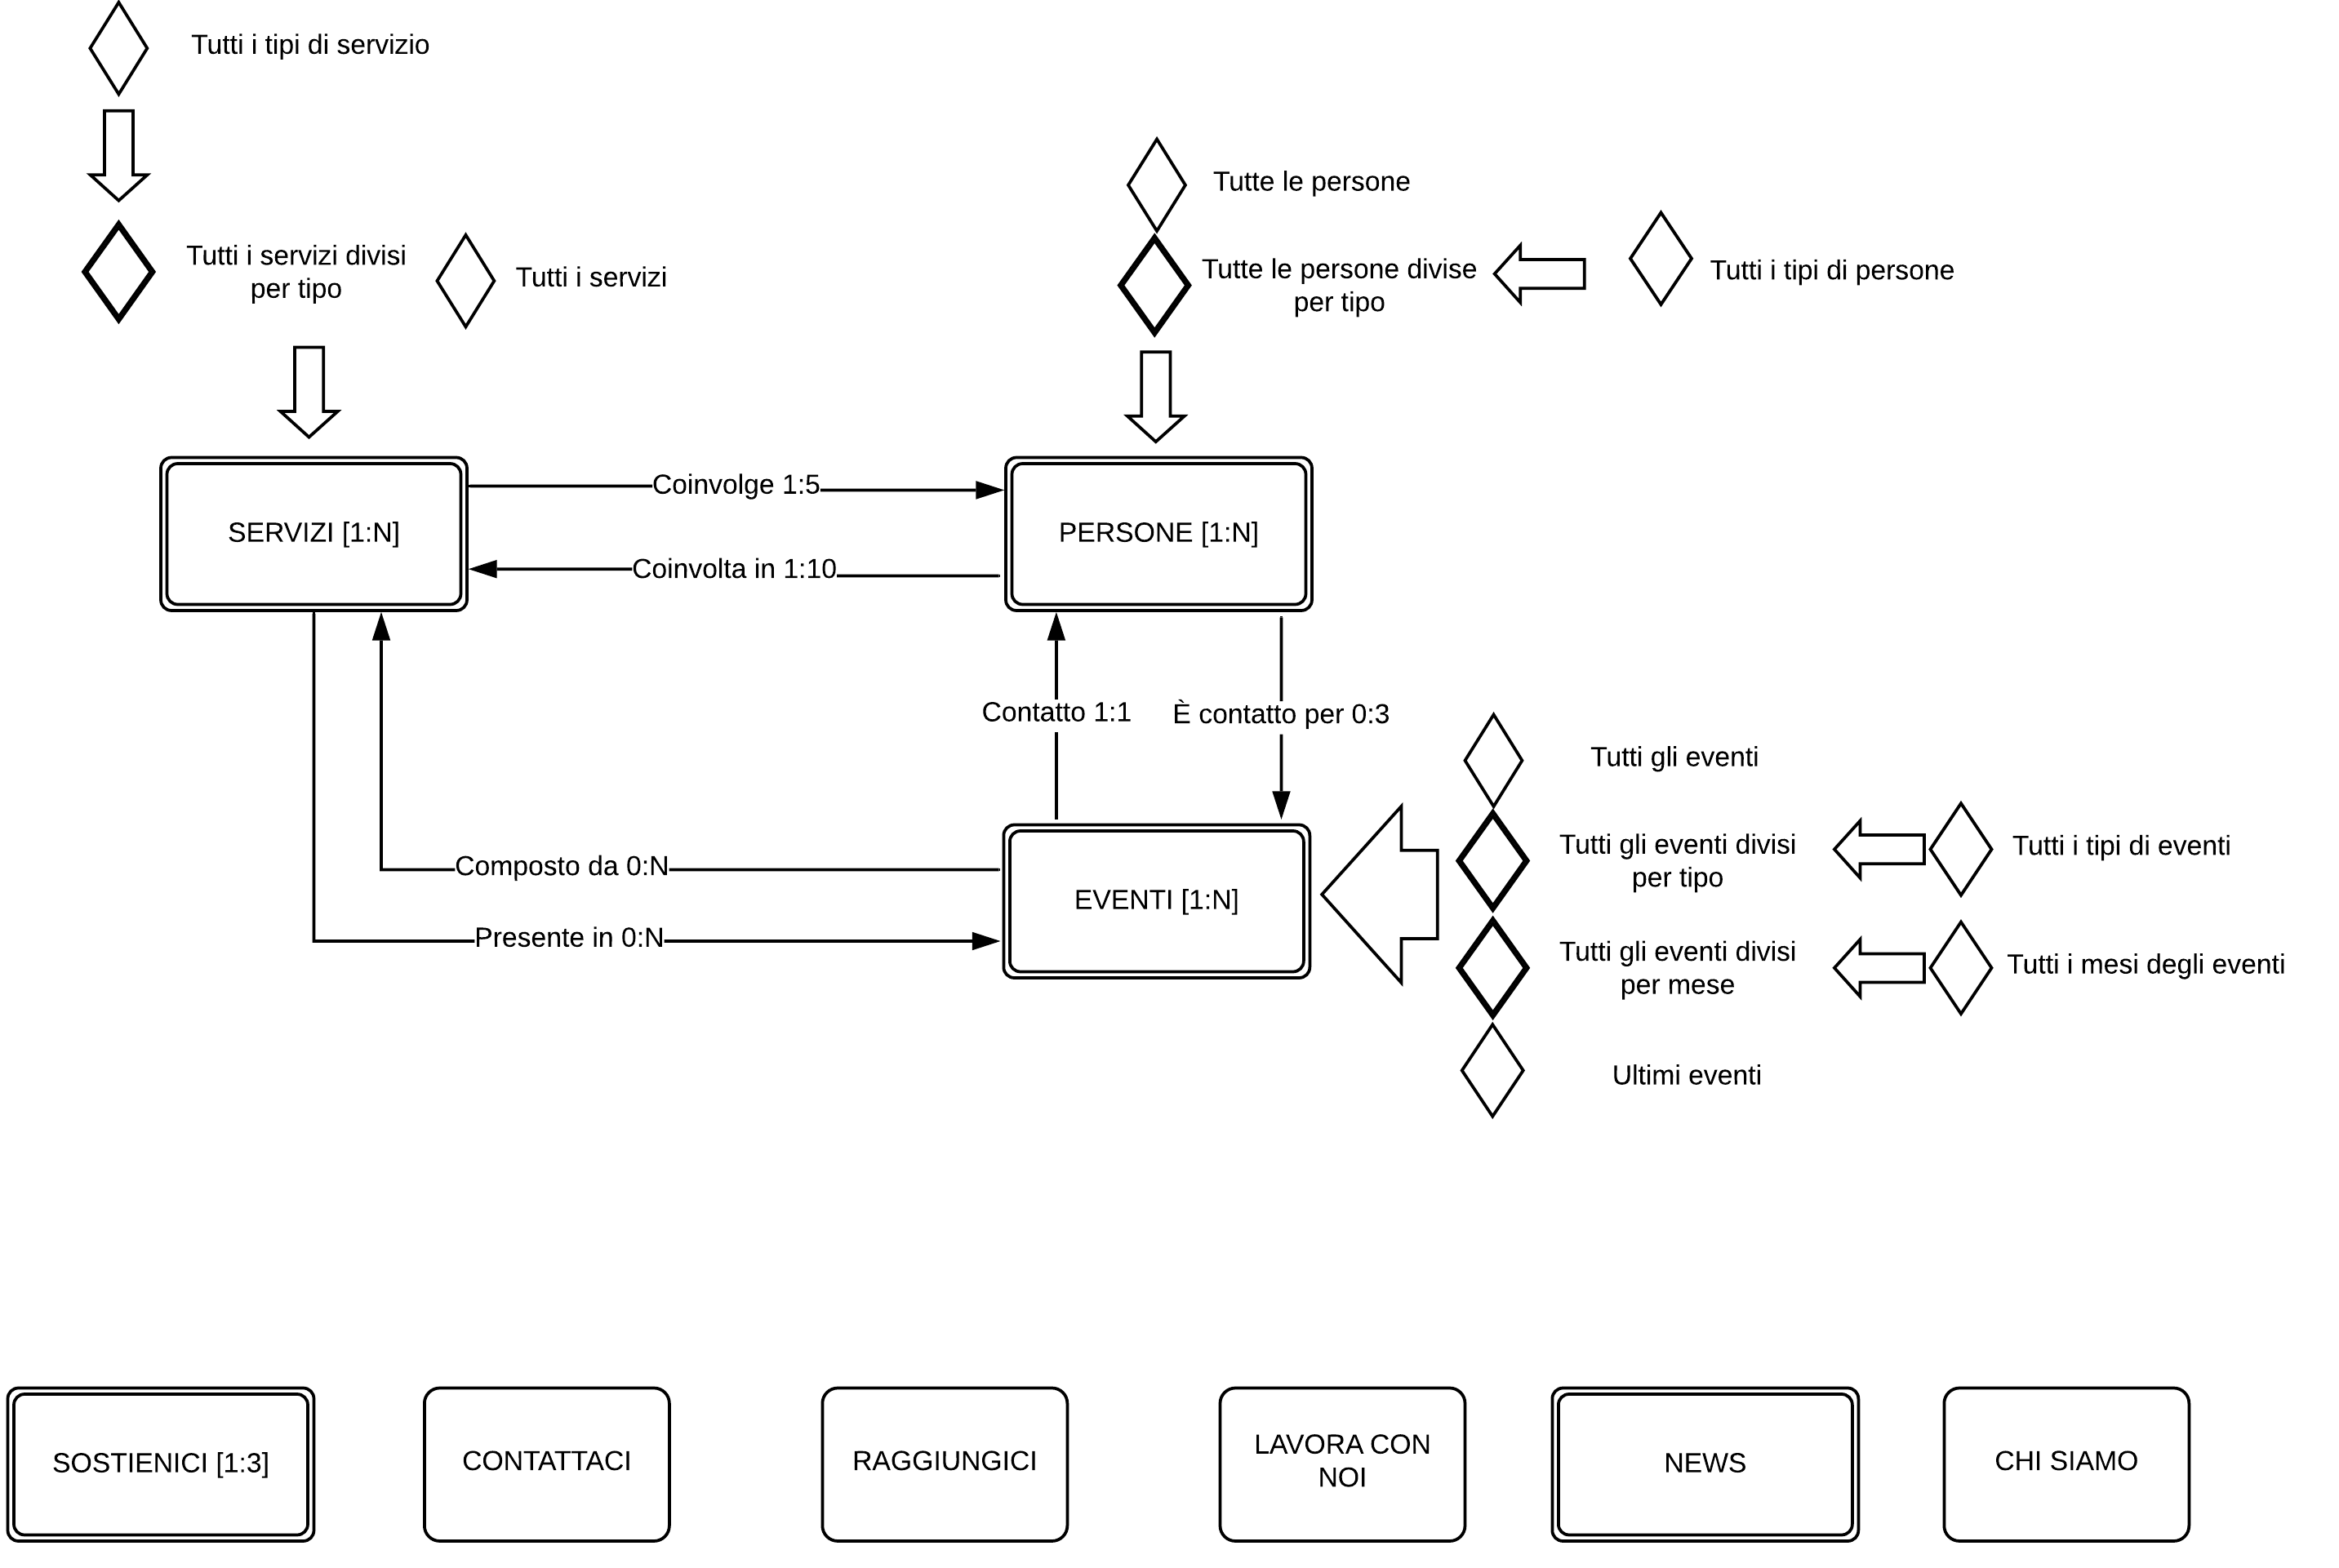
\includegraphics[scale=0.6]{resources/images/c-idm.png}
    \end{figure}
    \section{P-IDM}
    \begin{figure}[H]
        \centering
        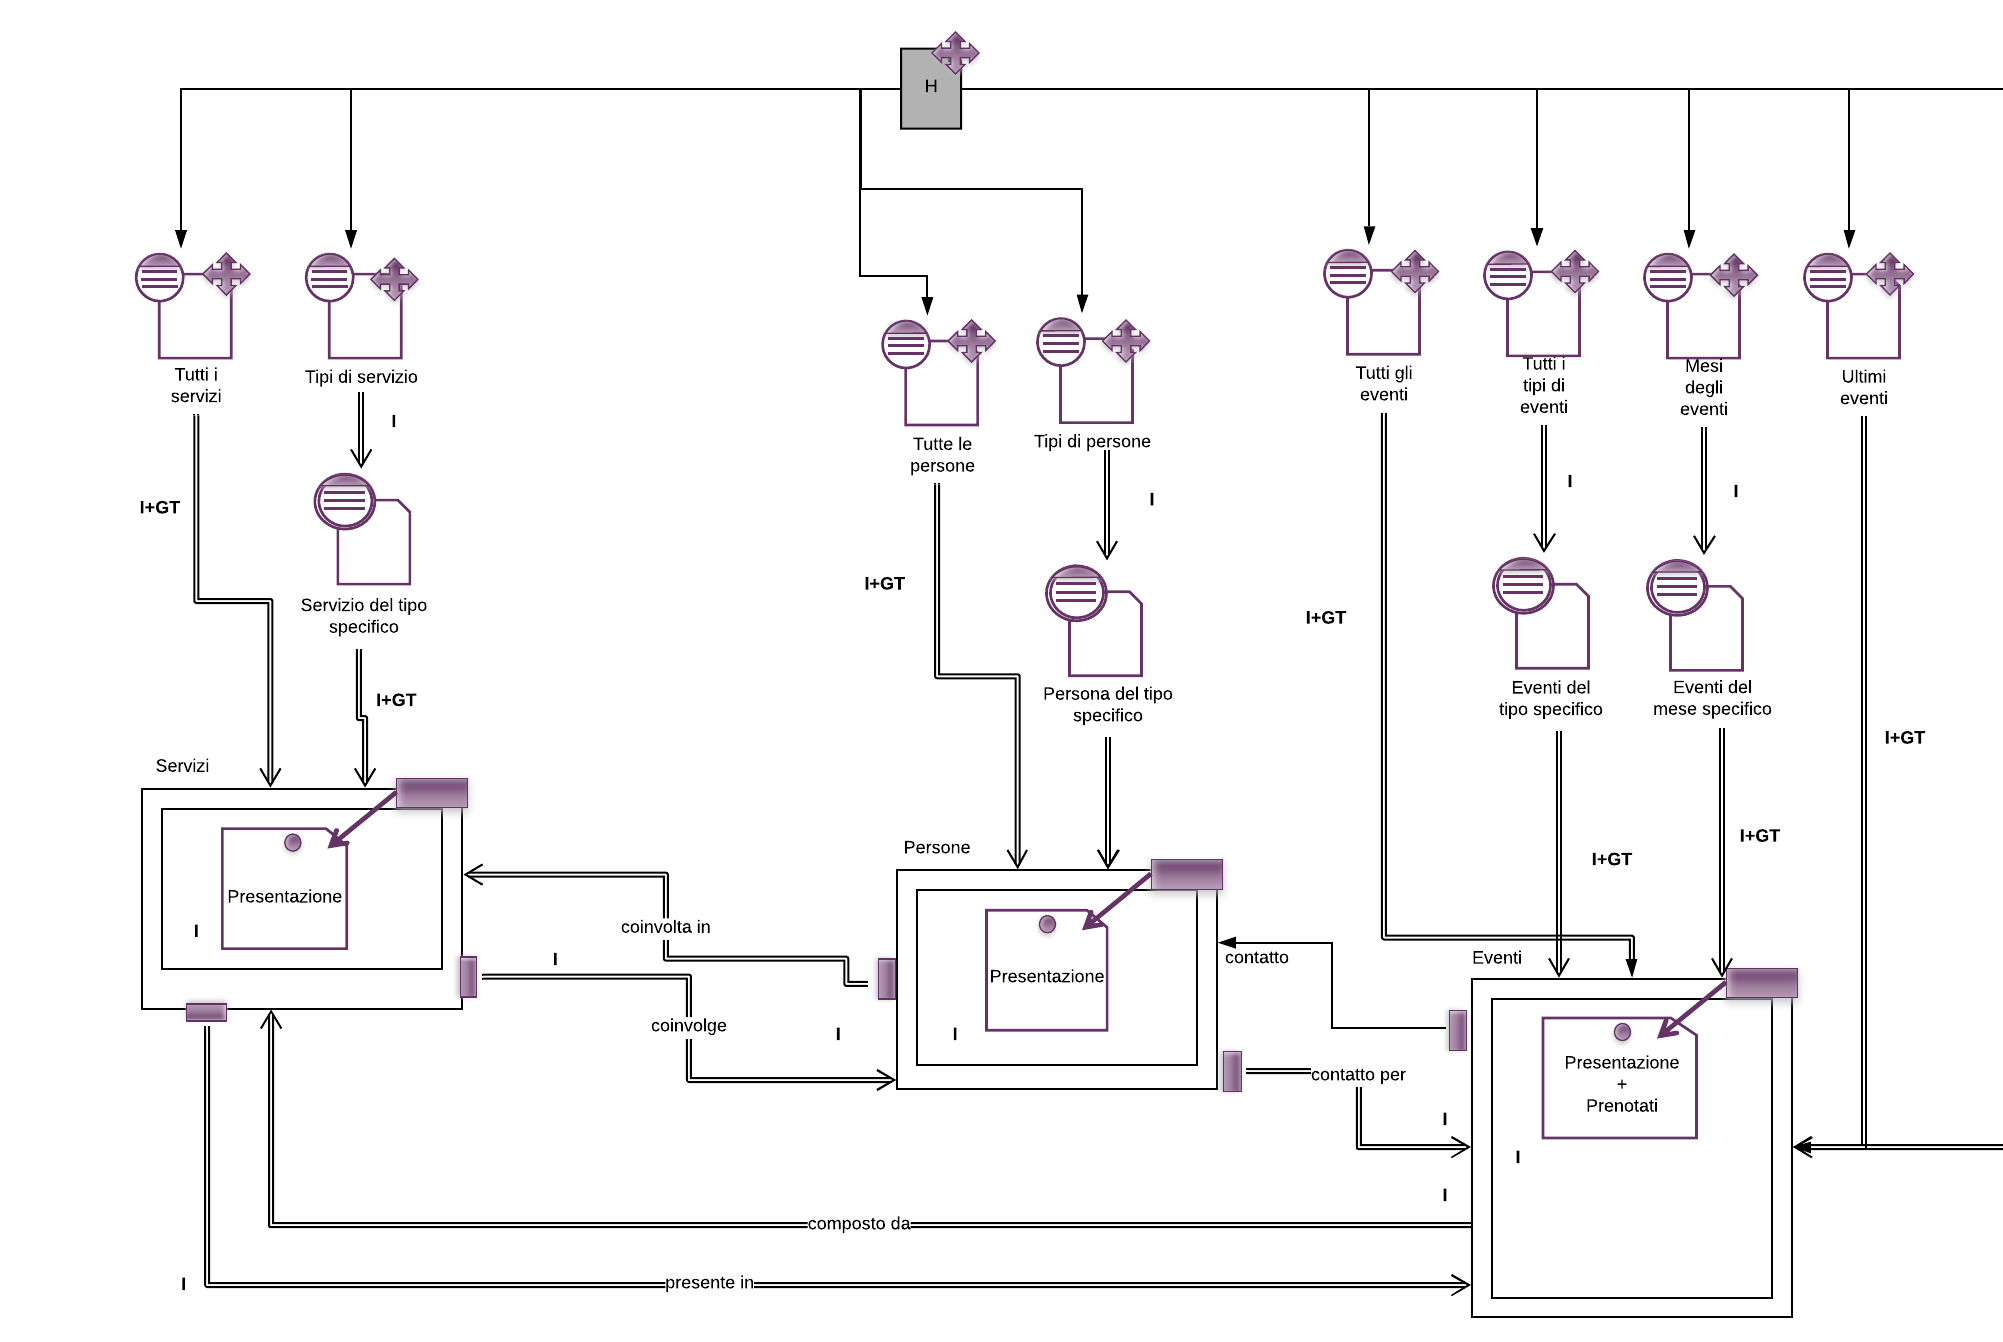
\includegraphics[scale=0.5]{resources/images/p-idm1.png}
    \end{figure}
    \begin{figure}[H]
        \centering
        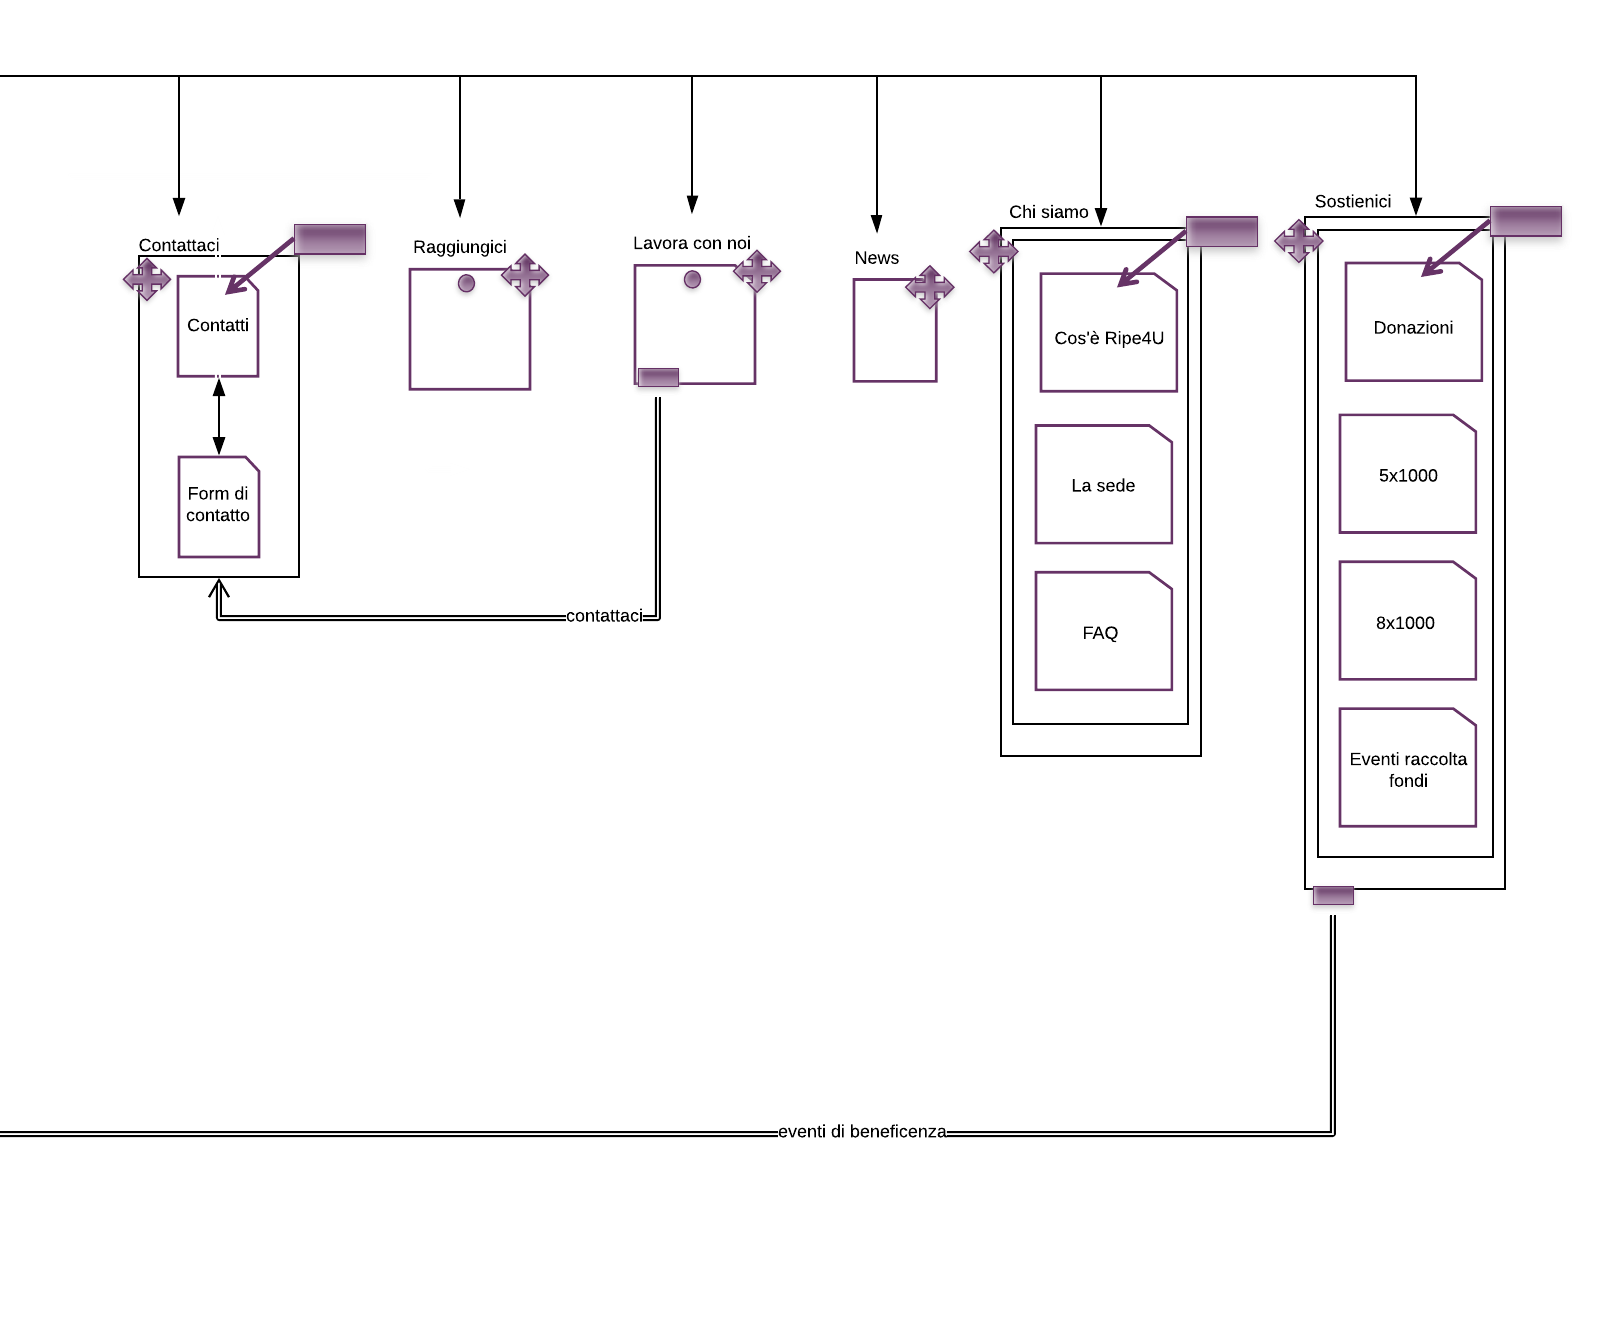
\includegraphics[scale=0.5]{resources/images/p-idm2.png}
    \end{figure}
   